\chapter{HAWK- Hybrid Question Answering using Linked Data}
\label{cha:app_hawk}


We present the evaluation of HAWK towards the \ac{QALD}-5 benchmark. The color codes can be resolved as follows:
\begin{itemize}
\item Yellow indicates that the ranking algorithms are not able to retrieve the correct SPARQL query out of the set of generated SPARQL queries. 
\item Orange cells point out that one ranking algorithm performs worse than the other. 
\item Red indicates the inability to retrieve correct answer sets.
That is, HAWK is able to generate a set of SPARQL queries but among them none retrieves a correct answer set.
\item Blue rows describe questions where HAWK is unable to generate at least one SPARQL query. Thus, those questions semantics cannot be captured by the system yet due to missing surface forms for individuals, classes and properties or missing indexed full-text information.
\end{itemize}
{
\scriptsize
\scriptsize
\begin{longtable}{@{}lp{0.4\linewidth}lllllllll@{}}
\toprule
         &                                                                                                             & \multicolumn{3}{l}{{\bf Feature-based Ranking}}     & \multicolumn{3}{l}{{\bf Overlap-based Ranking}}                                   & \multicolumn{3}{l}{{\bf Optimal Ranking}}                                      \\ \midrule
{\bf ID} & {\bf Question}                                                                                              & {\bf R}                & {\bf P}              & {\bf F1}             & {\bf R}              & {\bf P}           & {\bf F1}          & {\bf R}             & {\bf P}          & {\bf F1}         \\\midrule
301      & Who was vice-president under the president who authorized atomic weapons against Japan during World War II? & \cellcolor[HTML]{FFFE65}0   & \cellcolor[HTML]{FFFE65}0    & \cellcolor[HTML]{FFFE65}0    & \cellcolor[HTML]{FFFE65}0 & \cellcolor[HTML]{FFFE65}0 & \cellcolor[HTML]{FFFE65}0 & 1                        & 1                        & 1                        \\
303      & Which anti-apartheid activist was born in Mvezo?                                                            & \cellcolor[HTML]{F8A102}0   & \cellcolor[HTML]{F8A102}0    & \cellcolor[HTML]{F8A102}0    & 1                         & 0.5                       & 0.67                      & 1                        & 0.5                      & 0.67                     \\
305      & Which recipients of the Victoria Cross died in the Battle of Arnhem?                                        & \cellcolor[HTML]{F8A102}0   & \cellcolor[HTML]{F8A102}0    & \cellcolor[HTML]{F8A102}0    & 0.5                       & 0.33                      & 0.4                       & 0.5                      & 0.5                      & 0.5                      \\
306      & Where did the first man in space die?                                                                       & \cellcolor[HTML]{FFFE65}0   & \cellcolor[HTML]{FFFE65}0    & \cellcolor[HTML]{FFFE65}0    & \cellcolor[HTML]{FFFE65}0 & \cellcolor[HTML]{FFFE65}0 & \cellcolor[HTML]{FFFE65}0 & 1                        & 1                        & 1                        \\
308      & Which members of the Wu-Tang Clan took their stage name from a movie?                                       & \cellcolor[HTML]{F8A102}0.5 & \cellcolor[HTML]{F8A102}0.08 & \cellcolor[HTML]{F8A102}0.14 & 1                         & 0.17                      & 0.29                      & 0.5                      & 0.5                      & 0.5                      \\
309      & Which writers had influenced the philosopher that refused a Nobel Prize?                                    & \cellcolor[HTML]{FFFE65}0   & \cellcolor[HTML]{FFFE65}0    & \cellcolor[HTML]{FFFE65}0    & \cellcolor[HTML]{FFFE65}0 & \cellcolor[HTML]{FFFE65}0 & \cellcolor[HTML]{FFFE65}0 & 1                        & 1                        & 1                        \\
311      & Who composed the music for the film that depicts the early life of Jane Austin?                             & \cellcolor[HTML]{FE0000}   & \cellcolor[HTML]{FE0000}    & \cellcolor[HTML]{FE0000}    & \cellcolor[HTML]{FE0000} & \cellcolor[HTML]{FE0000} & \cellcolor[HTML]{FE0000} & \cellcolor[HTML]{FE0000} & \cellcolor[HTML]{FE0000} & \cellcolor[HTML]{FE0000} \\
314      & Which horses did The Long Fellow ride?                                                                      & \cellcolor[HTML]{FFFE65}0   & \cellcolor[HTML]{FFFE65}0    & \cellcolor[HTML]{FFFE65}0    & \cellcolor[HTML]{FFFE65}0 & \cellcolor[HTML]{FFFE65}0 & \cellcolor[HTML]{FFFE65}0 & 0.86                     & 1                        & 0.92                     \\
315      & Of the people that died of radiation in Los Alamos, whose death was an accident?                            & \cellcolor[HTML]{FFFE65}0   & \cellcolor[HTML]{FFFE65}0    & \cellcolor[HTML]{FFFE65}0    & \cellcolor[HTML]{FFFE65}0 & \cellcolor[HTML]{FFFE65}0 & \cellcolor[HTML]{FFFE65}0 & 0.5                      & 1                        & 0.67                     \\
316      & Which building owned by the Bank of America was featured in the TV series MegaStructures?                   & \cellcolor[HTML]{FE0000}   & \cellcolor[HTML]{FE0000}    & \cellcolor[HTML]{FE0000}    & \cellcolor[HTML]{FE0000} & \cellcolor[HTML]{FE0000} & \cellcolor[HTML]{FE0000} & \cellcolor[HTML]{FE0000} & \cellcolor[HTML]{FE0000} & \cellcolor[HTML]{FE0000} \\
317      & Which buildings in art deco style did Shreve, Lamb and Harmon design?                                       & 1                           & 0.33                         & 0.5                          & \cellcolor[HTML]{F8A102}0 & \cellcolor[HTML]{F8A102}0 & \cellcolor[HTML]{F8A102}0 & 1                        & 0.33                     & 0.5                      \\
318      & Which birds are protected under the National Parks and Wildlife Act?                                        & 0.67                        & 0.67                         & 0.67                         & 0.67                      & 0.67                      & 0.67                      & 0.67                     & 0.67                     & 0.67                     \\
319      & Which country did the first known photographer of snowflakes come from?                                     & \cellcolor[HTML]{FFFE65}0   & \cellcolor[HTML]{FFFE65}0    & \cellcolor[HTML]{FFFE65}0    & \cellcolor[HTML]{FFFE65}0 & \cellcolor[HTML]{FFFE65}0 & \cellcolor[HTML]{FFFE65}0 & 1                        & 1                        & 1                        \\
320      & List all the battles commanded by the lover of Cleopatra.                                                   & \cellcolor[HTML]{FFFE65}0   & \cellcolor[HTML]{FFFE65}0    & \cellcolor[HTML]{FFFE65}0    & \cellcolor[HTML]{FFFE65}0 & \cellcolor[HTML]{FFFE65}0 & \cellcolor[HTML]{FFFE65}0 & 0.23                     & 0.42                     & 0.29                     \\
322      & Which actress starring in the TV series Friends owns the production company Coquette Productions?           & \cellcolor[HTML]{FFFE65}0   & \cellcolor[HTML]{FFFE65}0    & \cellcolor[HTML]{FFFE65}0    & \cellcolor[HTML]{FFFE65}0 & \cellcolor[HTML]{FFFE65}0 & \cellcolor[HTML]{FFFE65}0 & 1                        & 1                        & 1                        \\
323      & Gaborone is the capital of which country member of the African Union?                                       & 1                           & 1                            & 1                            & 1                         & 1                         & 1                         & 1                        & 1                        & 1                        \\
326      & For which movie did the daughter of Francis Ford Coppola receive an Oscar?                                  & \cellcolor[HTML]{FE0000}   & \cellcolor[HTML]{FE0000}    & \cellcolor[HTML]{FE0000}    & \cellcolor[HTML]{FE0000} & \cellcolor[HTML]{FE0000} & \cellcolor[HTML]{FE0000} & \cellcolor[HTML]{FE0000} & \cellcolor[HTML]{FE0000} & \cellcolor[HTML]{FE0000} \\
327      & Which city does the first person to climb all 14 eight-thousanders come from?                               & \cellcolor[HTML]{BBDAFF}    & \cellcolor[HTML]{BBDAFF}     & \cellcolor[HTML]{BBDAFF}     & \cellcolor[HTML]{BBDAFF}  & \cellcolor[HTML]{BBDAFF}  & \cellcolor[HTML]{BBDAFF}  & \cellcolor[HTML]{BBDAFF} & \cellcolor[HTML]{BBDAFF} & \cellcolor[HTML]{BBDAFF} \\
328      & At which college did the only American actor that received the César Award study?                           & \cellcolor[HTML]{FE0000}   & \cellcolor[HTML]{FE0000}    & \cellcolor[HTML]{FE0000}    & \cellcolor[HTML]{FE0000} & \cellcolor[HTML]{FE0000} & \cellcolor[HTML]{FE0000} & \cellcolor[HTML]{FE0000} & \cellcolor[HTML]{FE0000} & \cellcolor[HTML]{FE0000} \\
332      & What is the native city of Hollywood's highest-paid actress?                                                & \cellcolor[HTML]{BBDAFF}    & \cellcolor[HTML]{BBDAFF}     & \cellcolor[HTML]{BBDAFF}     & \cellcolor[HTML]{BBDAFF}  & \cellcolor[HTML]{BBDAFF}  & \cellcolor[HTML]{BBDAFF}  & \cellcolor[HTML]{BBDAFF} & \cellcolor[HTML]{BBDAFF} & \cellcolor[HTML]{BBDAFF} \\
333      & In which city does the former main presenter of the Xposé girls live?                                       & \cellcolor[HTML]{FE0000}   & \cellcolor[HTML]{FE0000}    & \cellcolor[HTML]{FE0000}    & \cellcolor[HTML]{FE0000} & \cellcolor[HTML]{FE0000} & \cellcolor[HTML]{FE0000} & \cellcolor[HTML]{FE0000} & \cellcolor[HTML]{FE0000} & \cellcolor[HTML]{FE0000} \\
334      & Who plays Phileas Fogg in the adaptation of Around the World in 80 Days directed by Buzz Kulik?             & \cellcolor[HTML]{FFFE65}0   & \cellcolor[HTML]{FFFE65}0    & \cellcolor[HTML]{FFFE65}0    & \cellcolor[HTML]{FFFE65}0 & \cellcolor[HTML]{FFFE65}0 & \cellcolor[HTML]{FFFE65}0 & 1                        & 1                        & 1                        \\
335      & Who is the front man of the band that wrote Coffee \& TV?                                                   & \cellcolor[HTML]{FE0000}   & \cellcolor[HTML]{FE0000}    & \cellcolor[HTML]{FE0000}    & \cellcolor[HTML]{FE0000} & \cellcolor[HTML]{FE0000} & \cellcolor[HTML]{FE0000} & \cellcolor[HTML]{FE0000} & \cellcolor[HTML]{FE0000} & \cellcolor[HTML]{FE0000} \\
336      & Which Chinese-speaking country is a former Portguese colony?                                                & \cellcolor[HTML]{BBDAFF}    & \cellcolor[HTML]{BBDAFF}     & \cellcolor[HTML]{BBDAFF}     & \cellcolor[HTML]{BBDAFF}  & \cellcolor[HTML]{BBDAFF}  & \cellcolor[HTML]{BBDAFF}  & \cellcolor[HTML]{BBDAFF} & \cellcolor[HTML]{BBDAFF} & \cellcolor[HTML]{BBDAFF} \\
337      & What is the largest city in the county in which Faulkner spent most of his life?                            & \cellcolor[HTML]{BBDAFF}    & \cellcolor[HTML]{BBDAFF}     & \cellcolor[HTML]{BBDAFF}     & \cellcolor[HTML]{BBDAFF}  & \cellcolor[HTML]{BBDAFF}  & \cellcolor[HTML]{BBDAFF}  & \cellcolor[HTML]{BBDAFF} & \cellcolor[HTML]{BBDAFF} & \cellcolor[HTML]{BBDAFF} \\
340      & A landmark of which city is the home of the Mona Lisa?                                                      & \cellcolor[HTML]{FE0000}   & \cellcolor[HTML]{FE0000}    & \cellcolor[HTML]{FE0000}    & \cellcolor[HTML]{FE0000} & \cellcolor[HTML]{FE0000} & \cellcolor[HTML]{FE0000} & \cellcolor[HTML]{FE0000} & \cellcolor[HTML]{FE0000} & \cellcolor[HTML]{FE0000} \\
\hline
51       & Where was the "Father of Singapore" born?                                                                   & \cellcolor[HTML]{BBDAFF}    & \cellcolor[HTML]{BBDAFF}     & \cellcolor[HTML]{BBDAFF}     & \cellcolor[HTML]{BBDAFF}  & \cellcolor[HTML]{BBDAFF}  & \cellcolor[HTML]{BBDAFF}  & \cellcolor[HTML]{BBDAFF} & \cellcolor[HTML]{BBDAFF} & \cellcolor[HTML]{BBDAFF} \\
52       & Which Secretary of State was significantly involved in the United States' dominance of the Caribbean?       & \cellcolor[HTML]{FE0000}   & \cellcolor[HTML]{FE0000}    & \cellcolor[HTML]{FE0000}    & \cellcolor[HTML]{FE0000} & \cellcolor[HTML]{FE0000} & \cellcolor[HTML]{FE0000} & \cellcolor[HTML]{FE0000} & \cellcolor[HTML]{FE0000} & \cellcolor[HTML]{FE0000} \\
53       & Who is the architect of the tallest building in Japan?                                                      & \cellcolor[HTML]{BBDAFF}    & \cellcolor[HTML]{BBDAFF}     & \cellcolor[HTML]{BBDAFF}     & \cellcolor[HTML]{BBDAFF}  & \cellcolor[HTML]{BBDAFF}  & \cellcolor[HTML]{BBDAFF}  & \cellcolor[HTML]{BBDAFF} & \cellcolor[HTML]{BBDAFF} & \cellcolor[HTML]{BBDAFF} \\
55       & In which city where Charlie Chaplin's half brothers born?                                                   & \cellcolor[HTML]{BBDAFF}    & \cellcolor[HTML]{BBDAFF}     & \cellcolor[HTML]{BBDAFF}     & \cellcolor[HTML]{BBDAFF}  & \cellcolor[HTML]{BBDAFF}  & \cellcolor[HTML]{BBDAFF}  & \cellcolor[HTML]{BBDAFF} & \cellcolor[HTML]{BBDAFF} & \cellcolor[HTML]{BBDAFF} \\
56       & Which German mathematicians were members of the von Braun rocket group?                                     & \cellcolor[HTML]{FE0000}   & \cellcolor[HTML]{FE0000}    & \cellcolor[HTML]{FE0000}    & \cellcolor[HTML]{FE0000} & \cellcolor[HTML]{FE0000} & \cellcolor[HTML]{FE0000} & \cellcolor[HTML]{FE0000} & \cellcolor[HTML]{FE0000} & \cellcolor[HTML]{FE0000} \\
57       & Which writers converted to Islam?                                                                           & \cellcolor[HTML]{BBDAFF}    & \cellcolor[HTML]{BBDAFF}     & \cellcolor[HTML]{BBDAFF}     & \cellcolor[HTML]{BBDAFF}  & \cellcolor[HTML]{BBDAFF}  & \cellcolor[HTML]{BBDAFF}  & \cellcolor[HTML]{BBDAFF} & \cellcolor[HTML]{BBDAFF} & \cellcolor[HTML]{BBDAFF} \\
59       & Which movie by the Coen brothers stars John Turturro in the role of a New York City playwright?             & 1.00                        & 1.00                         & 1.00                         & 1.00                      & 1.00                      & 1.00                      & 1.00                     & 1.00                     & 1.00                     \\
60       & Which of the volcanoes that erupted in 1550 is still active?                                                & \cellcolor[HTML]{BBDAFF}    & \cellcolor[HTML]{BBDAFF}     & \cellcolor[HTML]{BBDAFF}     & \cellcolor[HTML]{BBDAFF}  & \cellcolor[HTML]{BBDAFF}  & \cellcolor[HTML]{BBDAFF}  & \cellcolor[HTML]{BBDAFF} & \cellcolor[HTML]{BBDAFF} & \cellcolor[HTML]{BBDAFF} \\ \bottomrule


\caption{Detailed results of HAWK at the QALD-5 challenge. R stands for Recall, P for Precision and F1 for F-measure.}
\label{tab:eval_qal5_detail}
\end{longtable}
}
Additionally, we show the detailed evaluation of the influence of different entity annotation systems towards the \ac{QALD}-4 benchmark, task hybrid questions, training on our hybrid \ac{QA} system, see Figure~\ref{chahawk:fig:EntityAnnotators}.
\begin{figure}[htb!]
\centering
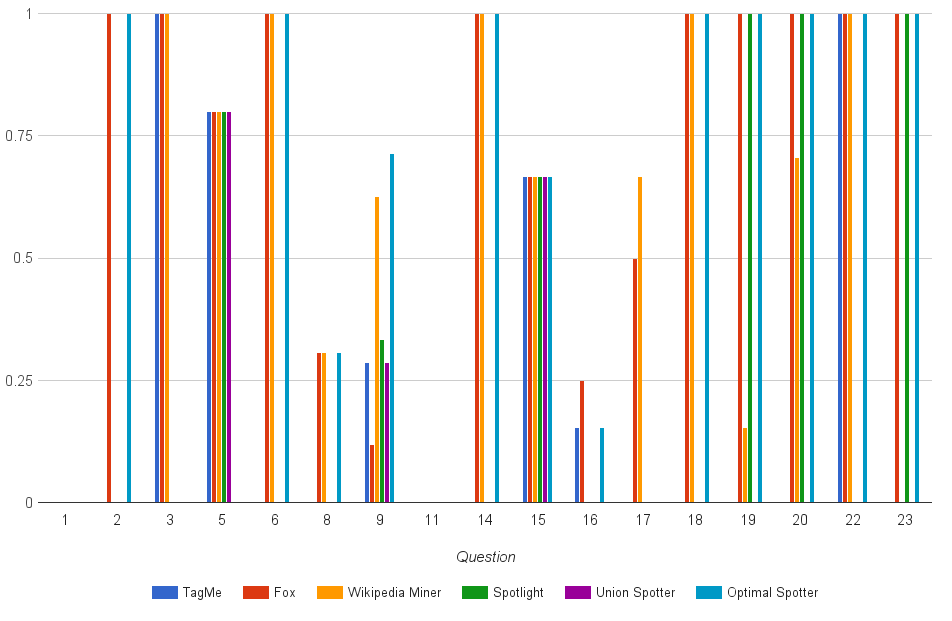
\includegraphics[width=\linewidth]{Appendix/fig/bars}
\caption{Entity annotations systems performance with optimal ranking.}
\label{chahawk:fig:EntityAnnotators}
\end{figure}
